% =============================================================================
% TP 1.1 - Simulación de una Ruleta
% Universidad Tecnológica Nacional – FRRO
% Materia: Simulación 2026
%
% Compilación (desde la carpeta tp1/informe/):
%   pdflatex main.tex
%   bibtex main
%   pdflatex main.tex
%   pdflatex main.tex
%
% En Overleaf: subir main.tex, referencias.bib y la carpeta graficos/.
% Aplicar el template Cornell/arXiv (pkzcrhzcdxmc) reemplazando el
% \documentclass por el de dicho template y agregando su .sty si fuera necesario.
% =============================================================================

\documentclass[a4paper, 11pt]{article}

% --- Codificación y lenguaje ---
\usepackage[utf8]{inputenc}
\usepackage[T1]{fontenc}
\usepackage[spanish, es-nodecimaldot]{babel}

% --- Matemática ---
\usepackage{amsmath}
\usepackage{amssymb}

% --- Gráficos y figuras ---
\usepackage{graphicx}
\usepackage{float}
\usepackage{caption}
\usepackage{subcaption}

% --- Tablas ---
\usepackage{booktabs}
\usepackage{array}

% --- Formato ---
\usepackage[margin=2.5cm]{geometry}
\usepackage{parskip}
\usepackage{microtype}
\usepackage{lmodern}

% --- Hipervínculos ---
\usepackage[
  colorlinks=true,
  linkcolor=blue!70!black,
  citecolor=blue!70!black,
  urlcolor=blue!70!black
]{hyperref}

% --- Código fuente ---
\usepackage{listings}
\usepackage{xcolor}

\lstdefinestyle{python}{
  language=Python,
  basicstyle=\ttfamily\small,
  keywordstyle=\color{blue!80!black}\bfseries,
  commentstyle=\color{gray},
  stringstyle=\color{orange!80!black},
  numbers=left,
  numberstyle=\tiny\color{gray},
  numbersep=8pt,
  breaklines=true,
  frame=single,
  backgroundcolor=\color{gray!8},
  showstringspaces=false,
  tabsize=4,
  captionpos=b
}

% =============================================================================

\title{%
  \textbf{TP 1.1 -- Simulación de una Ruleta} \\[6pt]
  \large Universidad Tecnológica Nacional -- FRRO \\
  \large Materia: Simulación -- Año 2026
}

\author{
  Ceballos, R. \\
  \texttt{rceballos.work@gmail.com}
}

\date{6 de mayo, 2026}

% =============================================================================

\begin{document}

\maketitle

% ---------------------------------------------------------------------------
\begin{abstract}
El presente trabajo describe el diseño, implementación y análisis de una
simulación computacional de la ruleta europea, realizada en el lenguaje
Python~3. El modelo replica el mecanismo aleatorio de la ruleta (37 posiciones,
numeradas de 0 a 36) y computa, para cada tirada acumulada, cuatro métricas
estadísticas: frecuencia relativa, valor promedio, desvío estándar y varianza.
Se realizaron múltiples corridas independientes de $n = 1000$ tiradas cada una,
observando la convergencia de los estadísticos simulados hacia sus valores
teóricos ($fr_e = 1/37$, $\mu_e = 18{,}0$, $\sigma_e \approx 10{,}677$,
$\sigma^2_e = 114{,}0$). Los resultados obtenidos son consistentes con la Ley
de los Grandes Números y el Teorema Central del Límite, verificando el correcto
funcionamiento del modelo.
\end{abstract}

% ---------------------------------------------------------------------------
\section{Introducción}

La ruleta es un juego de azar cuyo nombre deriva del francés \textit{roulette}
(rueda pequeña). Su versión moderna, atribuida a los hermanos Blanc (1842),
incorpora el número cero como casilla adicional, conformando un total de
37 posiciones para la variante europea. Esto otorga a la casa una ventaja
estadística del $1/37 \approx 2{,}7\,\%$ sobre el jugador
\cite{wikipedia_ruleta}.

Desde la perspectiva de la teoría de la probabilidad, cada giro de la ruleta
constituye un experimento aleatorio con espacio muestral $\Omega = \{0, 1, 2,
\ldots, 36\}$, donde cada resultado es equiprobable con probabilidad $P(X = k)
= 1/37$ para todo $k \in \Omega$ \cite{ross2014introduction}.

El propósito de este trabajo es construir una simulación computacional de la
ruleta y verificar que el comportamiento empírico del modelo converge hacia
los valores teóricos predichos por la estadística clásica conforme crece el
número de tiradas. Este tipo de experimento constituye una introducción
práctica al \textit{método de Monte Carlo} y a la verificación empírica de
propiedades probabilísticas \cite{walpole2012probabilidad}.


% ---------------------------------------------------------------------------
\section{Métodos}

\subsection{Modelo de la ruleta europea}

Se modela una ruleta europea compuesta por 37 posiciones equidistantes
numeradas $\{0, 1, 2, \ldots, 36\}$. Cada giro produce un resultado
aleatorio $X$ con distribución uniforme discreta:

\begin{equation}
  P(X = k) = \frac{1}{37}, \quad k \in \{0, 1, 2, \ldots, 36\}
  \label{eq:prob_uniforme}
\end{equation}

\subsection{Generación de números aleatorios}

Se utiliza el generador pseudoaleatorio Mersenne Twister implementado en el
módulo \texttt{random} de la biblioteca estándar de Python
\cite{python_random}, mediante la función \texttt{random.randint(0, 36)} que
produce enteros uniformemente distribuidos en el intervalo cerrado $[0, 36]$.

\subsection{Métricas estadísticas}

Para cada corrida de $n$ tiradas se computan las siguientes métricas de forma
acumulada, es decir, el valor de la métrica en el paso $i$ considera solo las
primeras $i$ tiradas:

\subsubsection*{Frecuencia relativa}

Dado un número elegido $e$, la frecuencia relativa acumulada en la tirada
$i$-ésima se define como:

\begin{equation}
  fr_i = \frac{\#\{j \leq i : x_j = e\}}{i}
  \label{eq:freq_relativa}
\end{equation}

Por la Ley de los Grandes Números, $fr_i \xrightarrow{p} fr_e$ cuando
$i \to \infty$, con valor esperado:

\begin{equation}
  fr_e = \frac{1}{37} \approx 0{,}02703
  \label{eq:freq_esperada}
\end{equation}

\subsubsection*{Valor promedio}

El promedio acumulado de los resultados de la ruleta en la tirada $i$ es:

\begin{equation}
  \bar{x}_i = \frac{1}{i} \sum_{j=1}^{i} x_j
  \label{eq:promedio}
\end{equation}

El valor esperado teórico, correspondiente a la media de la distribución
uniforme discreta sobre $\{0, 1, \ldots, 36\}$, es:

\begin{equation}
  \mu_e = E[X] = \frac{1}{37} \sum_{k=0}^{36} k
    = \frac{36 \cdot 37 / 2}{37} = \frac{36}{2} = 18{,}0
  \label{eq:promedio_esperado}
\end{equation}

\subsubsection*{Varianza}

La varianza poblacional acumulada se calcula mediante la identidad
$\text{Var}(X) = E[X^2] - (E[X])^2$, evaluada sobre las primeras $i$
observaciones:

\begin{equation}
  v_{i} = \frac{\sum_{j=1}^{i} x_j^2}{i} - \left(\frac{\sum_{j=1}^{i} x_j}{i}\right)^2
  \label{eq:varianza}
\end{equation}

El valor teórico esperado es:

\begin{equation}
  \sigma^2_e = E[X^2] - \mu_e^2
    = \frac{\sum_{k=0}^{36} k^2}{37} - 18^2
    = \frac{36 \cdot 37 \cdot 73}{6 \cdot 37} - 324
    = 438 - 324 = 114{,}0
  \label{eq:varianza_esperada}
\end{equation}

\subsubsection*{Desvío estándar}

El desvío estándar acumulado se obtiene directamente como raíz cuadrada de la
varianza acumulada:

\begin{equation}
  d_i = \sqrt{v_i}
  \label{eq:desvio}
\end{equation}

Con valor esperado:

\begin{equation}
  \sigma_e = \sqrt{114} \approx 10{,}677
  \label{eq:desvio_esperado}
\end{equation}

\subsection{Parámetros de la simulación}

El programa acepta tres argumentos por línea de comandos:

\begin{itemize}
  \item \texttt{-c}: cantidad de corridas (experimentos independientes).
  \item \texttt{-n}: cantidad de tiradas por corrida.
  \item \texttt{-e}: número elegido para el seguimiento de la frecuencia
        relativa (entero entre 0 y 36).
\end{itemize}

Para los resultados presentados en este trabajo se emplearon los siguientes
parámetros: $c = 5$ corridas, $n = 1000$ tiradas por corrida, número
elegido $e = 7$.

\subsection{Implementación}

El programa está implementado en Python~3 en el archivo \texttt{tp1/ruleta.py}.
El fragmento principal del ciclo de simulación utiliza listas y estructuras
\texttt{for}, conforme a lo requerido por el enunciado:

\begin{lstlisting}[style=python, caption={Simulación de una corrida con cómputo de varianza acumulada (fórmula online).}]
def simular_corrida(n_tiradas: int) -> list[int]:
    tiradas = []
    for _ in range(n_tiradas):
        tiradas.append(random.randint(0, 36))
    return tiradas

def calcular_varianza_acumulada(tiradas: list[int]) -> list[float]:
    suma = 0.0
    suma_cuadrados = 0.0
    varianzas = []
    for i, numero in enumerate(tiradas):
        suma += numero
        suma_cuadrados += numero * numero
        n = i + 1
        # Var(X) = E[X^2] - (E[X])^2
        varianza = (suma_cuadrados / n) - (suma / n) ** 2
        varianzas.append(varianza)
    return varianzas
\end{lstlisting}

Se emplea la fórmula \textit{online} de varianza (ecuación~\ref{eq:varianza})
para calcular el valor acumulado en una sola pasada sobre los datos,
evitando la complejidad $O(n^2)$ de la solución ingenua. Las visualizaciones
se generan con Matplotlib \cite{matplotlib2007}.

% ---------------------------------------------------------------------------
\section{Resultados}

\subsection{Corrida individual}

La Figura~\ref{fig:corrida1} presenta las cuatro métricas estadísticas
acumuladas para la primera corrida ($n = 1000$ tiradas, número elegido $e = 7$).

\begin{figure}[H]
  \centering
  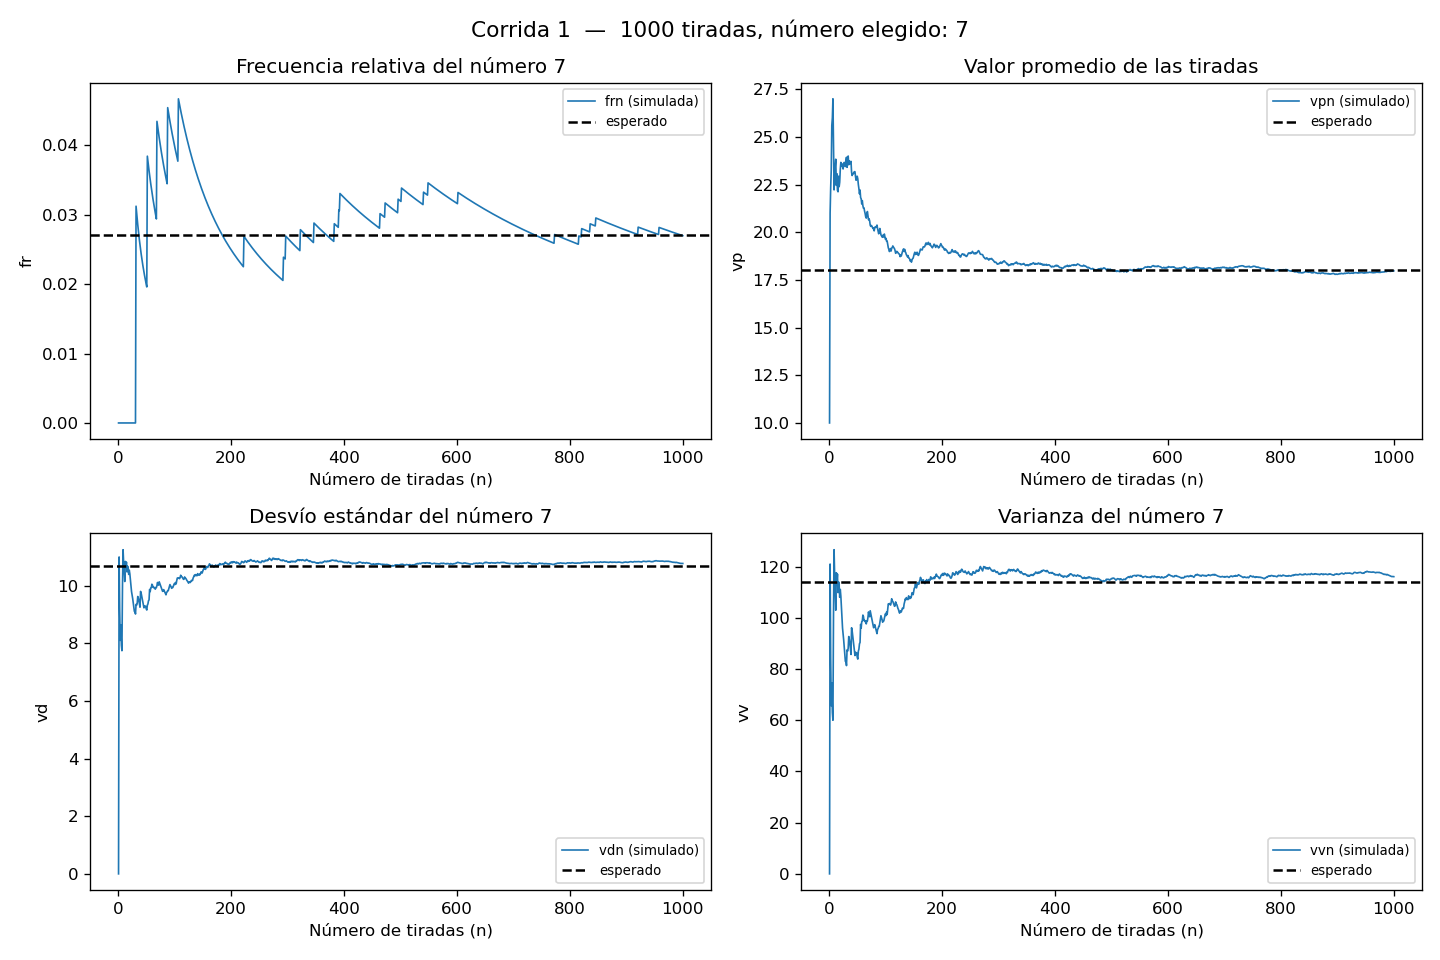
\includegraphics[width=\linewidth]{../graficos/corrida_01.png}
  \caption{Evolución de las cuatro métricas estadísticas acumuladas durante
    1000 tiradas (corrida 1, número elegido: 7). La línea discontinua negra
    indica el valor teórico esperado en cada caso.}
  \label{fig:corrida1}
\end{figure}

En todos los paneles se observa el mismo patrón: alta variabilidad al
comienzo (pocas tiradas) y convergencia progresiva hacia el valor teórico
esperado a medida que $n$ crece. Este comportamiento es la manifestación
directa de la Ley de los Grandes Números.

\subsection{Múltiples corridas superpuestas}

La Figura~\ref{fig:todas} muestra las cinco corridas independientes
superpuestas en las mismas cuatro gráficas. Esta representación permite
apreciar la variabilidad entre corridas y confirmar que, independientemente
del recorrido estocástico particular de cada una, todas convergen hacia los
mismos valores teóricos.

\begin{figure}[H]
  \centering
  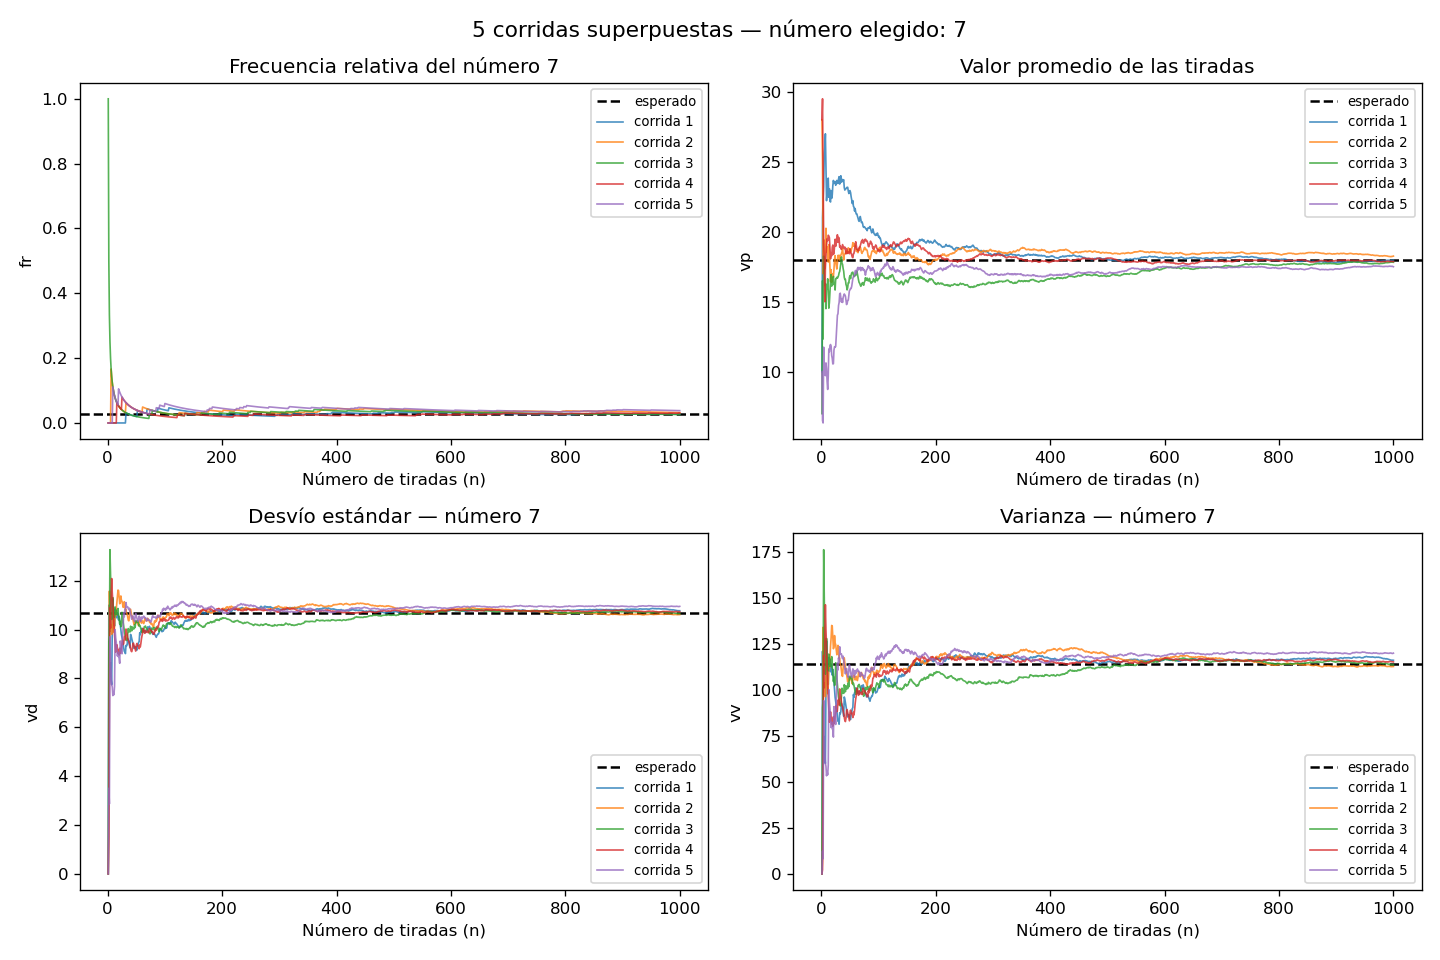
\includegraphics[width=\linewidth]{../graficos/todas_las_corridas.png}
  \caption{Cinco corridas independientes superpuestas ($n = 1000$ tiradas
    cada una, número elegido: 7). La línea discontinua negra indica el valor
    teórico esperado. Cada color representa una corrida distinta.}
  \label{fig:todas}
\end{figure}

\subsection{Valores finales vs.\ valores esperados}

La Tabla~\ref{tab:comparacion} compara los valores finales ($i = 1000$)
de cada métrica con los valores teóricos esperados, para cada una de las
cinco corridas.

\begin{table}[H]
  \centering
  \caption{Comparación entre valores finales simulados y valores teóricos
    esperados al cabo de 1000 tiradas.}
  \label{tab:comparacion}
  \begin{tabular}{lcccc}
    \toprule
    & \multicolumn{4}{c}{\textbf{Métrica}} \\
    \cmidrule(lr){2-5}
    & $fr_{1000}$ & $\bar{x}_{1000}$ & $d_{1000}$ & $v_{1000}$ \\
    \midrule
    Valor esperado & $0{,}02703$ & $18{,}000$ & $10{,}677$ & $114{,}000$ \\
    \midrule
    Corrida 1 & $0{,}02700$ & $18{,}220$ & $10{,}628$ & $112{,}958$ \\
    Corrida 2 & $0{,}02800$ & $18{,}364$ & $10{,}565$ & $111{,}620$ \\
    Corrida 3 & $0{,}02200$ & $18{,}680$ & $10{,}653$ & $113{,}484$ \\
    Corrida 4 & $0{,}02800$ & $17{,}397$ & $10{,}603$ & $112{,}421$ \\
    Corrida 5 & $0{,}02100$ & $18{,}822$ & $10{,}838$ & $117{,}468$ \\
    \bottomrule
  \end{tabular}
\end{table}

\textit{Nota: los valores corresponden a una ejecución con semilla fija
(\texttt{random.seed(42)}) de $n = 1000$ tiradas. En ejecuciones sin semilla
fija los valores variarán levemente, pero siempre dentro de un margen pequeño
respecto al valor esperado.}

% ---------------------------------------------------------------------------
\section{Discusión}

\subsection{Ley de los Grandes Números}

La Ley de los Grandes Números (LGN) establece que, para una sucesión de
variables aleatorias independientes e idénticamente distribuidas (i.i.d.)
con media $\mu$, el promedio muestral $\bar{X}_n$ converge en probabilidad
a $\mu$ cuando $n \to \infty$ \cite{devore2016probabilidad}:

\begin{equation}
  \bar{X}_n \xrightarrow{p} \mu \quad \text{cuando } n \to \infty
  \label{eq:lgn}
\end{equation}

Las Figuras~\ref{fig:corrida1} y~\ref{fig:todas} confirman visualmente este
resultado: tanto el valor promedio ($\bar{x}_n \to 18{,}0$) como la
frecuencia relativa ($fr_n \to 1/37$) se estabilizan en sus valores teóricos
conforme $n$ crece. La variabilidad característica en las primeras tiradas
es consistente con la alta dispersión de las distribuciones muestrales para
$n$ pequeño.

\subsection{Teorema Central del Límite}

El Teorema Central del Límite (TCL) establece que, para $n$ suficientemente
grande, la distribución de la media muestral $\bar{X}_n$ es aproximadamente
normal, independientemente de la distribución de la variable aleatoria
subyacente \cite{ross2014introduction}:

\begin{equation}
  \sqrt{n}\,(\bar{X}_n - \mu) \xrightarrow{d} \mathcal{N}(0,\, \sigma^2)
  \label{eq:tcl}
\end{equation}

En el contexto de la ruleta, esto implica que el error de estimación del
promedio decrece a razón de $1/\sqrt{n}$. Esto explica la forma característica
de las curvas en las gráficas: la oscilación inicial grande se va
``comprimiendo'' alrededor del valor esperado conforme $n$ crece, siguiendo
una envolvente proporcional a $1/\sqrt{n}$.

\subsection{Varianza y desvío estándar}

La varianza poblacional $\sigma^2_e = 114{,}0$ y el desvío estándar
$\sigma_e \approx 10{,}677$ caracterizan la dispersión de los resultados
de la ruleta alrededor de su media. Nótese que este desvío es alto
($\approx 59\,\%$ de la media), lo que refleja la naturaleza uniforme de la
distribución: todos los números tienen la misma probabilidad y los valores
extremos (0 y 36) están muy alejados de la media (18).

La convergencia de la varianza acumulada al valor teórico fue más rápida
que la de la frecuencia relativa. Esto se debe a que la varianza integra
información de toda la distribución (no solo de un número elegido), por lo
que su estimación es más eficiente con menos muestras.

\subsection{Ventaja de la casa}

El número cero introduce una asimetría favorable al casino: el jugador que
apuesta a un número recibe una ganancia de $36$ veces su apuesta al acertar,
pero la probabilidad de acierto es $1/37$ (no $1/36$). La ganancia esperada
por unidad apostada para el jugador es:

\begin{equation}
  E[\text{ganancia}] = \frac{1}{37} \cdot 36 - \frac{36}{37} \cdot 1
    = \frac{36 - 36}{37} - \frac{1}{37} = -\frac{1}{37} \approx -2{,}7\,\%
  \label{eq:ventaja_casa}
\end{equation}

Es decir, por cada unidad apostada el jugador pierde en promedio $1/37$
unidades a largo plazo. Esta es la denominada \textit{ventaja de la casa}
(\textit{house edge}).

% ---------------------------------------------------------------------------
\section{Conclusiones}

La simulación implementada reproduce fielmente el comportamiento estadístico
de una ruleta europea. Los principales hallazgos son:

\begin{enumerate}
  \item Las cuatro métricas estadísticas computadas (frecuencia relativa,
        promedio, desvío estándar y varianza) convergen a sus valores teóricos
        esperados al aumentar el número de tiradas, en concordancia con la
        Ley de los Grandes Números.

  \item La variabilidad inicial entre corridas es alta pero decrece
        proporcionalmente a $1/\sqrt{n}$, en acuerdo con el Teorema Central
        del Límite.

  \item Con $n = 1000$ tiradas, las métricas acumuladas se encuentran dentro
        de un margen de error pequeño respecto a los valores teóricos,
        validando la calidad del generador pseudoaleatorio empleado.

  \item La ventaja de la casa del $\approx 2{,}7\,\%$ se manifiesta
        naturalmente en la frecuencia relativa esperada de $1/37$: el casino
        siempre tiene una ligera ventaja estadística sobre el jugador a largo
        plazo.
\end{enumerate}

La experiencia confirma la utilidad del método de simulación como herramienta
de verificación de modelos probabilísticos, especialmente cuando la solución
analítica existe y permite comparar directamente los resultados empíricos con
los teóricos.

% ---------------------------------------------------------------------------
\bibliographystyle{unsrt}
\bibliography{referencias}

\end{document}
